\documentclass[11pt]{article}
\usepackage[margin=1in]{geometry}
\usepackage{amsmath,amssymb,amsfonts,mathtools}
\usepackage{booktabs,array,tabularx}
\usepackage{graphicx}
\usepackage{lmodern}
\usepackage[protrusion=true,expansion=false]{microtype}
\usepackage[colorlinks=true,linkcolor=blue,citecolor=blue,urlcolor=blue]{hyperref}
\usepackage{url}
\usepackage{setspace}
\usepackage[labelfont=bf,font=small]{caption}
\setstretch{1.05}
\setlength{\parskip}{0pt}
\setlength{\tabcolsep}{4pt}
\newcommand{\hd}[1]{\medskip\par\noindent\textbf{#1}\par\nobreak\vspace{2pt}\noindent\ignorespaces}
\newcommand{\mz}{\ensuremath{m/z}}
\graphicspath{{./}{cheminformatics/manuscript/}{manuscript/}}

\title{\vspace{-2em}\bfseries A metadata-matched binned baseline halves the apparent peak-level advantage in MS/MS substructure prediction}
\author{Xulin Pan\textsuperscript{1}\thanks{Correspondence: \texttt{xulinpanias@gmail.com}}
\quad Chuanming Wang\textsuperscript{2}\\[4pt]
\small \textsuperscript{1}The Pennsylvania State University, University Park, PA, USA\\
\small \textsuperscript{2}School of Biological and Food Engineering, Honghe University, Mengzi, China}
\date{}

\begin{document}
\maketitle

\subsection*{Abstract}
\small
Machine-learning methods for tandem mass spectrometry (MS/MS) increasingly replace fixed-width binned intensity vectors with models that consume individual peaks at full mass precision, and gains over binned baselines are often discussed as evidence for the richer spectral representation. Such comparisons can also change the encoder and the acquisition information available to the model. We examine these sources separately in MS/MS substructure prediction. Our openly licensed corpus contains $414{,}992$ spectra from GNPS, MassBank and MoNA spanning $66$ instrument types, of which $372{,}200$ survive preprocessing. Across $10{,}058$ held-out molecules and three seeds, an unconditioned binned baseline trails a full-precision peak-token model by $+0.0579$ macro AUPRC. Supplying it with the acquisition covariates the peak-token arms already had raises it from $0.1130$ to $0.1418$, closing $+0.0288$ of that gap and leaving $+0.0291$. Within the same peak-token encoder, restoring full mass precision contributes $+0.0142$ (95\% target-resampling interval $+0.0097$ to $+0.0187$). The other $+0.0149$ separates the conditioned dense baseline from the rounded peak-token pipeline and therefore represents a broader token-encoder package rather than a pure encoder effect. An attention-free token arm matches the attention-bearing arm ($-0.0023$, interval $-0.0066$ to $+0.0020$), though pooling and feed-forward width also differ, so this is a sensitivity comparison rather than a pure attention ablation. Hierarchical aggregation contributes $+0.0179$. A near-homogeneous second corpus reproduces the pattern. The conclusion is methodological: comparator construction and metadata availability affect the attribution of gains as much as mass resolution does.
\normalsize

\hd{Scientific contribution}
\small
We provide a rounding control that isolates the value of mass-axis precision within a fixed peak-token encoder, and a metadata-matched dense baseline that exposes a larger comparator confound. On the primary corpus, acquisition metadata alone accounts for roughly half of the apparent advantage of the full-precision peak-token model; after that correction, mass precision contributes $+0.0142$ macro AUPRC and the remaining dense-to-token pipeline change $+0.0149$. The study therefore supports a narrower but stronger claim than a conventional two-arm comparison: gains over binned baselines should not be attributed to spectral representation unless acquisition information and the relevant model changes are controlled explicitly.
\normalsize

\hd{Keywords}
\small Tandem mass spectrometry, structure annotation, spectral representation, mass defect, substructure prediction, ablation study, baseline design
\normalsize

\section*{Introduction}
Assigning a chemical structure to an MS/MS spectrum is a central challenge in untargeted metabolomics. Where the molecule appears in a reference library, the task can be approached by spectral matching, but many spectra acquired from biological extracts do not have an exact reference match \cite{hoffmann2022cosmic}. Computational annotation therefore relates a spectrum to candidate structures through in-silico fragmentation and scoring, as in MetFrag \cite{ruttkies2016metfrag}; prediction of structural fingerprints followed by database search, as in CSI:FingerID \cite{duhrkop2015csifingerid} and MIST \cite{goldman2023mist}; or learned spectral representations, as in MS2DeepScore \cite{huber2021ms2deepscore} and DreaMS \cite{bushuiev2025dreams}.

For much of the recent machine-learning literature, a spectrum has been discretised onto a fixed grid of bins and presented to a model as a dense vector. This convention originated in spectral library search, where bins wider than the instrument's mass error can make matching robust to calibration drift. A $0.5$~Da bin spans roughly $1{,}700$~ppm at $\mz=300$, whereas a modern time-of-flight instrument can operate at approximately $5$~ppm. Such binning therefore discards fine-scale information including mass defect, the difference between exact and nominal mass; for example, $\mathrm{C_5H_7^+}$ ($67.0542$) and $\mathrm{C_4H_3O^+}$ ($67.0178$) fall within the same $0.5$~Da bin despite distinct elemental compositions.

Modern systems increasingly avoid coarse binning. CSI:FingerID scores fragmentation trees over exact masses, MIST tokenises peaks by chemical formula, DreaMS operates on peak lists, and TransExION embeds nominal mass and mass defect in separate channels \cite{buithi2024transexion}. Recent work also benchmarks alternative MS/MS featurisations \cite{gine2026benchmarking} and explores the amount of mass resolution needed for chemical-similarity prediction \cite{dejonge2026cross}.

These two studies are the most direct empirical statements available about what mass precision is worth, and they point in different directions. Gin\'e et al.\ \cite{gine2026benchmarking} compare adaptive binning and spectrum hashing against learned embeddings across a large grid of models for structure annotation, and report that retrieval degrades markedly as the mass tolerance is relaxed. Working on chemical-similarity prediction rather than structure annotation, de Jonge et al.\ \cite{dejonge2026cross} settle on $0.1$~Da bins and report that finer bins did not improve performance. The disagreement is itself a reason to ask the question in a form that admits a clean answer. Both studies establish that representation matters; neither isolates which part of a pipeline causes a particular gain, because a benchmark measures each featurisation bundled with the encoder that reads it and therefore estimates a joint effect at many points rather than separating it at one.

The reason is structural. A dense binned vector and a sparse, variable-length peak set require different input interfaces, so moving from one to the other commonly changes the representation and encoder together. Additional differences can enter through training protocol, pooling and acquisition metadata. A two-arm comparison therefore estimates the joint difference between complete pipelines, not the causal contribution of the spectral representation alone.

We address this attribution problem in a controlled MS/MS substructure-prediction setting. Our key control quantises the mass axis inside the peak-token pipeline: peaks are snapped to the same $0.5$~Da grid used by the dense baseline, collisions are merged, and the resulting tokens are passed through the same peak-set encoder used for full-precision peaks. This makes the M1R-to-M1 contrast a direct test of mass-axis precision while holding the peak-token architecture fixed. We also correct an acquisition-metadata imbalance in the original dense baseline. Finally, we include an attention-free token sensitivity arm and hierarchical spectrum aggregation to place the mass-axis effect in context. We explicitly distinguish the contrasts that are clean one-factor interventions from those that remain composite.

\section*{Methods}
\hd{Corpora and splits}
Both corpora are drawn from the CASMI 2026 training corpus, an aggregation of eleven public and in-house MS/MS libraries whose \texttt{ingest\_lib} field records the source library. The primary source corpus is the openly licensed subset contributed by GNPS, MassBank and MoNA: $414{,}992$ spectra over $52{,}428$ structures, spanning $66$ instrument types and $112$ adducts. After filtering, $372{,}200$ spectra over $50{,}287$ structures and $24{,}627{,}256$ peaks remain for modelling. We distinguish these source and retained counts throughout.

The secondary corpus is a contiguous slice of two of the file's twenty-one row groups, containing $262{,}144$ spectra. Because the file is ordered by source library, this slice is not a random sample: it is $99.0\%$ one in-house library and $1.0\%$ another, and $99\%$ of spectra come from a single instrument (timsTOF), across two instrument types and sixteen adducts. We therefore use it as a deliberately contrasting sensitivity corpus rather than as an independent external replication dataset.

Spectra were retained if precursor $\mz<2{,}000$ and the reported precursor error was within $20$~ppm. Peaks were retained above $0.1\%$ of the base peak and below the precursor plus $1.5$~Da, capped at the $256$ most intense, with $\mz$ held in double precision throughout preprocessing.

Structures were assigned to five folds by grouping generic Murcko scaffolds, with acyclic structures falling back to grouping by their own identifier, and fold sizes balanced greedily. Folds 2--4 were used for fitting, fold 1 for model selection and fold 0 for final evaluation. Fold 0 contains $10{,}058$ molecules on the open corpus and $8{,}692$ on the single-library corpus. This design follows the generalisation-demanding practice used in MassSpecGym \cite{bushuiev2024massspecgym}, while retaining source-library selection specific to the present study.

\hd{Structural targets}
Each structure was decomposed with BRICS and represented by the presence or absence of each of the $512$ most frequent attachment-labelled fragments, with the vocabulary fitted on the training folds only. On the open corpus the target matrix is $99.3\%$ zero with a median of four positive targets per molecule. A total of $433$ targets have at least five held-out positives, at a mean prevalence of $0.0085$. The single-library corpus is less sparse ($97.1\%$ zero, median 17 positive targets, 477 scored targets, mean prevalence $0.0093$). Because the targets are highly imbalanced, macro AUPRC is the primary metric; macro AUROC, micro AUPRC and Brier score are secondary summaries.

\hd{Five-arm ablation ladder}
The five arms are ordered as M0, M1D, M1R, M1 and M2. The ladder is useful for decomposing the observed pipeline difference, but not every adjacent contrast is a pure one-factor intervention. In particular, M1R-to-M1 is a clean mass-axis intervention, whereas M0-to-M1D and M1D-to-M1R remain composite contrasts as described below.

\emph{M0, metadata-matched dense baseline.} Each spectrum is projected onto $2{,}048$ fragment bins and $2{,}048$ precursor-minus-fragment bins of width $0.5$~Da over $[0,1024)$, with square-root intensity accumulated within bins and the concatenated $4{,}096$-dimensional vector $L_2$-normalised. A two-layer perceptron encodes the vector. Collision energy, adduct, polarity and instrument embeddings are concatenated to the dense representation. This gives M0 access to the same acquisition variables as the peak-token arms, although the conditioning mechanism is not identical: the token encoder injects them through adaptive layer normalisation.

\emph{M1R, rounded peak-token control.} Each fragment mass $m$ is assigned to a cell by $\lfloor m/w \rfloor$, with $w=0.5$~Da, and moved to the cell centre. Peaks sharing a cell are merged by accumulating square-root intensity, matching the accumulator used by M0. The precursor is snapped to the same grid before the neutral loss is computed, preventing fine precursor mass from leaking back into the token representation. The resulting tokens pass through the same peak-token encoder used by M1. M1R and M1 have identical parameter counts ($712{,}336$) and differ only by whether mass quantisation is active. This is the principal representation control in the study.

\emph{M1D, attention-free token sensitivity arm.} M1D uses the same rounded peak masses and acquisition variables as M1R, but removes self-attention from the token blocks. Because a learned pooling token cannot aggregate independent position-wise tokens in the absence of attention, M1D uses masked-mean pooling. Removing attention also frees parameters, so its feed-forward layers were widened, yielding $714{,}528$ parameters versus $712{,}336$ for M1R. M1D therefore tests whether the attention-bearing configuration improves on an approximately capacity-matched attention-free token model; it does \emph{not} isolate a pure attention effect because pooling and feed-forward width also change.

\emph{M1, full-precision peak-token model.} M1 is identical to M1R except that mass quantisation is disabled, so the model receives the instrument-reported mass precision. The M1-to-M1R contrast therefore isolates the effect of mass-axis precision within a fixed encoder, pooling rule, training protocol and parameter count.

\emph{M2, hierarchical aggregation.} M2 is identical to M1 except that mean pooling over a molecule's spectra is replaced by a measurement model that weights each spectrum by a learned, acquisition-dependent precision. The M2-to-M1 contrast isolates the effect of this hierarchical aggregation module.

\hd{Peak encoding}
Each peak is encoded as a token. For a peak at $\mz=m$ in a spectrum with precursor mass $m^{\mathrm{prec}}$, we form a multi-scale sinusoidal embedding
\begin{equation}
\varphi_L(m)=\bigl[\sin(2\pi m/\lambda_1),\cos(2\pi m/\lambda_1),\ldots,\sin(2\pi m/\lambda_L),\cos(2\pi m/\lambda_L)\bigr]^\top,
\end{equation}
with $L=32$ wavelengths spaced geometrically from $2$~mDa to $10^3$~Da, applied to both fragment mass and neutral loss. The token also receives the explicit defect $\delta=m-\mathrm{round}(m)$, square-root and log-transformed intensity, and intensity rank. At a wavelength of $2$~mDa and $\mz=342$ the phase exceeds $10^6$, so the phase is evaluated in double precision and reduced modulo $2\pi$ before casting. Tokens are then encoded by a four-block Transformer, with acquisition covariates entering each block through adaptive layer normalisation.

\hd{Bin-width sweep}
To examine the precision scale continuously, we repeated the M1R construction at $w\in\{0.25,0.1,0.05,0.01\}$~Da, holding the encoder, parameter count, training schedule and seed fixed. Together with $w=0.5$ and full precision, this produces six mass-resolution settings. The sweep was run on the single-library corpus only and each intermediate width was trained once; it is therefore treated as exploratory except for the endpoints.

\hd{Training protocol}
Every arm was trained for 15 epochs with AdamW, a one-cycle learning-rate schedule peaking at $10^{-3}$, batches of 16 molecules, mixed precision and gradient clipping at 1.0. The objective was binary cross-entropy over the 512 BRICS-presence targets plus an auxiliary negative-binomial term on 88 functional-group counts. Checkpoints were selected by validation macro AUPRC. No hyperparameter search was performed for any arm. We note that this is not a symmetric choice: the schedule was selected for the peak-token Transformer and inherited unchanged by the dense baseline, so M0 and the token arms are not equidistant from their respective optima. The five ladder arms on the open corpus and four arms on the single-library corpus were each trained under seeds $\{2026,7,13\}$, for 27 ladder runs in total, in addition to the single-seed sweep runs.

\hd{Evaluation and uncertainty}
Macro AUPRC is reported over targets with at least five held-out positives. For paired contrasts, each target's average precision is first averaged over the three seeds; per-target differences are then computed and their mean is resampled over targets with 5,000 bootstrap draws. We refer to the resulting intervals as \emph{target-resampling intervals}. They describe variability across the scored target set after seed averaging; they do not incorporate uncertainty from alternative scaffold splits, and BRICS targets are not statistically independent because fragments co-occur. We therefore report seed-to-seed standard deviations separately and interpret the intervals descriptively rather than as complete uncertainty statements for a broader population of tasks.

\section*{Results}
\hd{Performance across the five-arm ladder}
Table~\ref{tab:arms} summarises the five arms on the open corpus. The metadata-matched M0 baseline reaches 0.1418 macro AUPRC, M1D 0.1590, M1R 0.1567, M1 0.1709 and M2 0.1888. The central representation contrast, M1 minus M1R, is therefore measured within an identical peak-token architecture. By contrast, M0-to-M1D and M1D-to-M1R should be read as composite pipeline comparisons rather than pure interface and attention effects.

\begin{table}[ht]
\centering
\caption{Five-arm ablation ladder on the open corpus. Macro AUPRC is evaluated on 10,058 held-out molecules and averaged over three seeds. Chance is 0.0085 over 433 scored targets. Pooling is separated into two axes because they differ between different pairs of arms: peak pooling within a spectrum distinguishes M1D from M1R, and spectrum pooling within a molecule distinguishes M2 from M1.}
\label{tab:arms}
\small
\begin{tabular}{lllllrrr}
\toprule
Arm & Mass axis & Encoder/interface & Peak pooling & Spectrum pooling & Parameters & Macro AUPRC & Seed SD\\
\midrule
M0 & 0.5 Da bins & dense vector, MLP & bin accumulation & mean & 1,172,752 & 0.1418 & 0.0013\\
M1D & 0.5 Da grid & peak tokens, attention-free & masked mean & mean & 714,528 & 0.1590 & 0.0024\\
M1R & 0.5 Da grid & peak tokens, attention-bearing & learned token & mean & 712,336 & 0.1567 & 0.0025\\
M1 & full precision & peak tokens, attention-bearing & learned token & mean & 712,336 & 0.1709 & 0.0022\\
M2 & full precision & peak tokens, attention-bearing & learned token & hierarchical & 829,584 & 0.1888 & 0.0015\\
\bottomrule
\end{tabular}
\end{table}

\begin{figure}[ht]
\centering
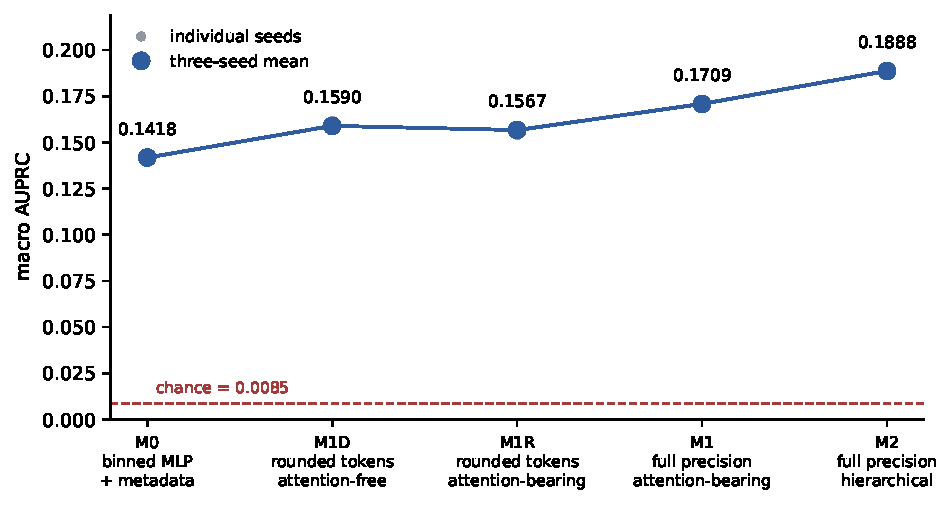
\includegraphics[width=0.93\linewidth]{figure1_arm_means.pdf}
\caption{Held-out macro AUPRC for the five arms on the open corpus. Large markers are three-seed means, small markers the individual seeds. The seeds are drawn because two of the increments compared below cannot be ordered: their difference changes sign across these runs.}
\label{fig:arms}
\end{figure}

\hd{Matching acquisition metadata closes half of the original two-arm gap}
The initial dense baseline did not use collision energy, adduct, polarity or instrument variables, whereas the peak-token models did. Adding the same acquisition variables to M0 by concatenating their embedding to the dense spectral vector raises M0 from 0.1130 to 0.1418, an improvement of $+0.0288$. Consequently, the apparent M1-to-M0 advantage falls from $+0.0579$ to $+0.0291$. Thus, about half of the original two-arm difference was attributable to unequal metadata availability rather than to mass precision or peak-token modelling. Because M0 and the peak-token arms inject the metadata through different mechanisms, we describe the corrected comparator as \emph{metadata matched}, not as mechanically identical in conditioning.

\hd{Mass precision and the rounded-token pipeline contribute similar numerical increments}
Against metadata-matched M0, M1 reaches 0.1709, a paired target-level gain of $+0.0291$ (95\% target-resampling interval $+0.0208$ to $+0.0371$), with 72.5\% of targets improved. The M1R control divides that numerical difference into $+0.0149$ for M1R minus M0 and $+0.0142$ for M1 minus M1R. The latter is a clean mass-axis effect because M1R and M1 are identical except for quantisation. The former is broader: it combines the change from dense-vector MLP to rounded peak tokens, the change in peak pooling, and differences in how acquisition covariates are injected. We therefore label it the \emph{rounded token-encoder package} effect rather than a pure encoder effect, reserving \emph{binned token-encoder package} for the corresponding contrast against the attention-free arm, $\mathrm{M1D}-\mathrm{M0}$.

The two increments are numerically similar in this experiment, and their difference changes sign across seeds. This supports the conclusion that the remaining performance difference cannot be attributed predominantly to mass precision. It does not establish that ``architecture'' and mass precision have equal causal effects in a design-independent sense.

\hd{The attention-bearing configuration provides no measurable advantage in the present sensitivity arm}
M1D minus M0 is $+0.0172$ ($+0.0102$ to $+0.0242$), while M1R minus M1D is $-0.0023$ ($-0.0066$ to $+0.0020$). Thus the attention-bearing rounded-token model does not outperform the attention-free rounded-token model in this comparison. We do not interpret the negative mean as evidence that attention is harmful. More importantly, M1D-to-M1R is not a pure attention intervention because the two arms also differ in pooling and feed-forward width. The appropriate conclusion is therefore limited to the configurations tested: adding the attention-bearing design did not produce a measurable gain over the approximately capacity-matched attention-free token model.

\begin{table}[ht]
\centering
\caption{Paired target-level contrasts on the open corpus. Intervals are bootstrap target-resampling intervals after averaging target AP across the three seeds. The first two contrasts are composite pipeline comparisons; M1--M1R and M2--M1 are the cleanest one-factor interventions.}
\label{tab:contrasts}
\small
\begin{tabularx}{\linewidth}{lXrrr}
\toprule
Contrast & Interpretation & $\Delta$ AUPRC & 95\% interval & Targets improved\\
\midrule
M1D $-$ M0 & binned token-encoder package & +0.0172 & [+0.0102, +0.0242] & 58.0\%\\
M1R $-$ M1D & attention-bearing vs attention-free configuration & -0.0023 & [-0.0066, +0.0020] & 54.3\%\\
M1R $-$ M0 & rounded token-encoder package & +0.0149 & [+0.0080, +0.0221] & 66.7\%\\
M1 $-$ M1R & mass-axis precision & +0.0142 & [+0.0097, +0.0187] & 64.9\%\\
M2 $-$ M1 & hierarchical aggregation & +0.0179 & [+0.0136, +0.0223] & 63.7\%\\
M1 $-$ M0 & joint token-pipeline and mass-axis difference & +0.0291 & [+0.0208, +0.0371] & 72.5\%\\
M2 $-$ M0 & all changes combined & +0.0470 & [+0.0377, +0.0566] & 73.9\%\\
\bottomrule
\end{tabularx}
\end{table}

\begin{figure}[ht]
\centering
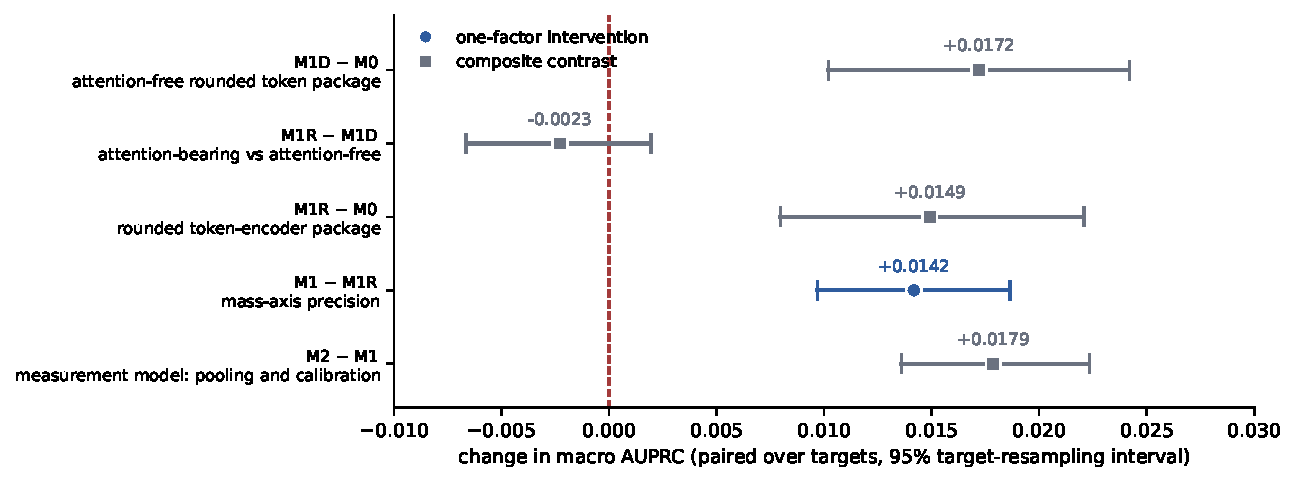
\includegraphics[width=0.88\linewidth]{figure2_contrasts.pdf}
\caption{Selected paired target-level contrasts on the open corpus, with $95\%$ target-resampling intervals. Contrasts drawn in grey are composite: the corresponding arms differ in more than the named factor, as described in Methods. Only the mass-axis and aggregation contrasts change a single component.}
\label{fig:contrasts}
\end{figure}

\hd{Observed ordering across seeds}
Hierarchical aggregation exceeds the M1R-minus-M0 token-encoder package in all three open-corpus seeds by $+0.0009$, $+0.0030$ and $+0.0049$, and exceeds the mass-axis effect in all three by $+0.0028$, $+0.0045$ and $+0.0037$. The same direction is observed for aggregation versus the token-encoder package in all three seeds on the single-library corpus. With only three seeds per corpus, we treat this as a consistent empirical ordering in these runs rather than as an established general ranking.

The token-encoder package and mass-axis increments cannot be ordered reliably. Their difference is $+0.0019$, $+0.0015$ and $-0.0012$ across the open-corpus seeds, and the sign also varies on the single-library corpus ($-0.0016$, $+0.0006$, $-0.0090$). The mass-axis contrast is the most reproducible of the main contrasts across open-corpus seeds, with an SD of 0.0004, compared with 0.0013 for M1R minus M0 and 0.0009 for aggregation.

\hd{Sensitivity analysis on a contrasting corpus}
The same ladder was evaluated on the near-homogeneous single-library corpus. Table~\ref{tab:corpora} compares the three principal increments. All are larger on the single-library corpus than on the open corpus, but the broad pattern remains: the mass-axis and rounded token-encoder increments are of similar order, and aggregation is also substantial. This cross-corpus consistency is informative, but the secondary corpus is not an independent external replication because it is a contiguous in-house slice of the same aggregate CASMI resource.

\begin{table}[ht]
\centering
\caption{Contrasts on the near-homogeneous single-library corpus and the open corpus. ``Token-encoder package'' denotes M1R--M0 and should not be interpreted as a pure encoder effect.}
\label{tab:corpora}
\small
\begin{tabular}{lrrrr}
\toprule
Contrast & Single library & SD & Open corpus & SD\\
\midrule
Token-encoder package (M1R--M0) & +0.0234 & 0.0002 & +0.0149 & 0.0013\\
Mass axis (M1--M1R) & +0.0268 & 0.0049 & +0.0142 & 0.0004\\
Aggregation (M2--M1) & +0.0322 & 0.0035 & +0.0179 & 0.0009\\
Share of M1--M0 assigned numerically to M1R--M0 & 46.7\% & -- & 51.3\% & --\\
Peaks absorbed at 0.5 Da in held-out spectra & 34.4\% & -- & 23.6\% & --\\
\bottomrule
\end{tabular}
\end{table}

The metadata correction also appears in both corpora: supplying acquisition covariates to M0 improves macro AUPRC by $+0.0288$ on the open corpus and $+0.0142$ on the single-library corpus. The larger gain in the more heterogeneous corpus is consistent with the idea that acquisition context becomes more valuable as experimental conditions diversify, but the present analysis does not isolate a causal relation between corpus heterogeneity and metadata value.

\hd{What binning removes}
On the open corpus's held-out spectra, 23.6\% of the $3{,}797{,}166$ peaks fall into a $0.5$~Da bin already occupied by another peak from the same spectrum and are therefore absorbed. The corresponding fraction on the single-library held-out spectra is 34.4\%. At $0.01$~Da the reported held-out absorption fractions fall to 2.9\% and 6.5\%, respectively. A merged peak also loses compositional discrimination: enumerating plausible CHNOS compositions within 10~ppm places 328 candidate fragment formulae inside a single $0.5$~Da bin at $\mz=300$, consistent with the dependence of formula ambiguity on mass tolerance described by Kind and Fiehn \cite{kind2007seven}.

Absorption falls with the grid on both corpora (Fig.~\ref{fig:absorption}), which is what makes the bin-width sweep below interpretable as a precision axis rather than an arbitrary reparameterisation. Absorption is reported throughout on each corpus's own held-out spectra; the same quantity computed over all retained spectra is $37.5\%$ rather than $34.4\%$ on the single-library corpus, and we quote the held-out figure because it matches the set on which the effects are measured.

The corpus that loses more peaks at 0.5~Da is also the corpus in which the mass-axis effect is larger ($34.4\%$ and $+0.0268$ versus $23.6\%$ and $+0.0142$). This association is descriptive and does not identify the mechanism. One plausible explanation is that the single-library corpus is almost entirely high-resolution timsTOF data, whereas the open corpus spans instruments of varying resolution. That explanation remains a hypothesis until the mass-axis effect is stratified directly by instrument resolution.

\begin{figure}[ht]
\centering
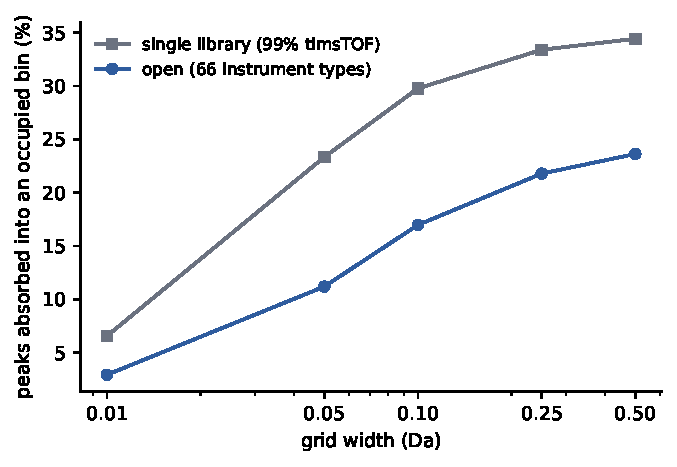
\includegraphics[width=0.62\linewidth]{figure3_absorption.pdf}
\caption{Fraction of peaks absorbed into an already-occupied bin, against grid width, on each corpus's own held-out spectra.}
\label{fig:absorption}
\end{figure}

\hd{Exploratory bin-width sweep}
On the single-library corpus, the single-seed sweep gives macro AUPRC values of 0.0867 at 0.5~Da, 0.0818 at 0.25~Da, 0.0801 at 0.1~Da, 0.0909 at 0.05~Da, 0.1030 at 0.01~Da and 0.1119 at full precision. The non-monotonic values at 0.25 and 0.1~Da are compatible with training noise in a single run and should not be interpreted as evidence that coarser grids are better. The 0.01~Da model closes approximately 65\% of the 0.5~Da-to-full-precision gap. Because each intermediate width was run once and only on one corpus, the apparent transition below 0.05~Da is exploratory rather than a transferable threshold.

\begin{table}[ht]
\centering
\caption{Single-seed bin-width sweep on the single-library corpus. Every arm uses the M1 encoder at an identical parameter count; only the width of the mass grid changes. The final column expresses each result as a share of the distance between the 0.5~Da arm and full precision.}
\label{tab:sweep}
\small
\begin{tabular}{lrr}
\toprule
Bin width (Da) & Macro AUPRC & Share of 0.5 Da gap closed\\
\midrule
0.5 & 0.0867 & 0\%\\
0.25 & 0.0818 & -19\%\\
0.1 & 0.0801 & -26\%\\
0.05 & 0.0909 & 17\%\\
0.01 & 0.1030 & 65\%\\
Full precision & 0.1119 & 100\%\\
\bottomrule
\end{tabular}
\end{table}

\section*{Discussion}
The main result is a reattribution of an apparent representation gain. A simple two-arm comparison between the original unconditioned binned baseline and the full-precision peak-token model yields $+0.0579$ macro AUPRC. Supplying the dense baseline with the acquisition covariates already available to the peak-token models accounts for $+0.0288$ of that difference. After metadata matching, the remaining M1-to-M0 difference is $+0.0291$.

Within the peak-token architecture, the rounding control gives the cleanest causal contrast in the study: restoring full mass precision contributes $+0.0142$. The remaining M1R-to-M0 difference is $+0.0149$, but it should not be described as a pure encoder effect because the two arms also differ in input interface and in how the acquisition metadata are injected. The robust conclusion is therefore not that ``encoder and mass axis are exactly equal,'' but that the apparent full-precision advantage is not dominated by mass resolution once the comparator receives the same acquisition variables.

The attention-free sensitivity arm leads to a similarly narrower interpretation than in the previous draft. M1R does not outperform M1D, but the arms differ in mean versus learned-token pooling and in feed-forward width in addition to attention. The experiment therefore shows that the tested Transformer-style attention-bearing configuration is not necessary to obtain the rounded-token performance observed here; it does not identify the isolated causal effect of self-attention. A future exact ablation should hold feed-forward width and pooling fixed while toggling only the attention operator.

These distinctions matter because the purpose of the study is attribution. When representation, interface, architecture and metadata availability move together, a performance increment belongs to the whole package unless the design contains an intervention that changes only one component. The rounding control satisfies that requirement for mass-axis precision. The metadata correction establishes a separate and practically important point: comparator inputs themselves can account for a performance difference as large as the modelling changes being studied.

The results should also be scoped to the present endpoint. The targets are 512 frequent BRICS fragments, not candidate-ranking accuracy, full molecular fingerprints or de-novo structure elucidation. The study therefore does not establish why CSI:FingerID, MIST, DreaMS, TransExION or other external systems outperform their own baselines. It provides a control strategy and an empirical warning that can be applied to those systems: when a paper attributes a gain to spectral representation, the comparator should receive matched acquisition information and the representation effect should be isolated within a fixed encoder whenever possible.

The contrasting single-library corpus is useful because it changes the acquisition regime substantially, but it should not be called an independent replication. The larger mass-axis increment on the nearly all-timsTOF corpus is compatible with the hypothesis that preserving reported mass precision is more valuable when the instrument genuinely supplies high-resolution measurements. That explanation is scientifically plausible but untested here. The appropriate next analysis is to stratify the M1-minus-M1R effect by instrument-resolution class using the saved held-out predictions, ideally without retraining.

The bin-width sweep is likewise suggestive rather than definitive. It indicates that a 0.01~Da grid recovers much of, but not all of, the full-precision advantage on the single-library corpus. This differs below 0.1~Da from the result reported by de Jonge et al. \cite{dejonge2026cross}. The tasks, architectures and training stochasticity differ, and the present sweep has only one seed at each intermediate width, so neither study alone settles a universal ``sufficient'' mass resolution.

\hd{Limitations}
The study has several limitations relevant to interpretation. First, three seeds per ladder arm are sufficient to show the observed seed-to-seed pattern but not to establish universal rankings among small effects. Second, the bootstrap intervals resample BRICS targets after seed averaging; they do not incorporate scaffold-split uncertainty and they treat correlated fragment targets as exchangeable. Third, the dense baseline and peak-token arms receive the same acquisition variables through different conditioning mechanisms, so M1R-to-M0 is not a pure architecture contrast. Fourth, M1D-to-M1R is not a pure attention contrast because pooling and feed-forward width also change. Fifth, the secondary corpus is a deliberately contrasting in-house slice rather than an external independent replication. Sixth, the instrument-resolution explanation is not tested directly. Seventh, the intermediate bin-width sweep is single-seed and single-corpus. Eighth, no arm was tuned, and the shared schedule was chosen for the token model rather than for the dense baseline; the metadata correction reported here, worth more than any contrast in the study, is direct evidence that M0 was not near its ceiling, so a learning-rate and width search for M0 alone could move the $+0.0149$ M1R-to-M0 increment again. Finally, the endpoint is BRICS substructure prediction; transfer to candidate retrieval or full structure annotation remains to be demonstrated.

Three additional experiments would most directly strengthen the attribution. A learning-rate and width search for M0 alone, reported against the untuned token arms, would make the remaining increments conservative rather than vulnerable. A metadata-matched dense baseline using a conditioning mechanism more analogous to the token model would test whether the $+0.0149$ M1R-to-M0 increment depends on how metadata are injected. An exact attention ablation with identical feed-forward width and identical pooling on both sides would replace the current sensitivity comparison with a true one-factor contrast.

\section*{Conclusion}
On the primary open corpus, an unconditioned $0.5$~Da binned baseline trails a full-precision peak-token model by $+0.0579$ macro AUPRC. Supplying the baseline with collision energy, adduct, polarity and instrument information raises its macro AUPRC from 0.1130 to 0.1418 and closes $+0.0288$ of that gap. Against this metadata-matched comparator, the remaining difference is $+0.0291$.

The cleanest representation result is obtained inside the peak-token architecture: restoring full mass precision contributes $+0.0142$ macro AUPRC. The numerically similar $+0.0149$ M1R-to-M0 increment belongs to a broader rounded token-encoder package, not to an isolated encoder effect. Likewise, the attention-bearing rounded-token configuration does not outperform the attention-free sensitivity arm, but the current design does not isolate attention alone. Hierarchical aggregation contributes $+0.0179$.

The practical conclusion is therefore about experimental design rather than a universal ranking of model components. In MS/MS substructure prediction, attribution depends strongly on how the comparator is constructed. Acquisition variables must be matched explicitly, and claims about mass representation should be supported by a within-architecture control such as quantising the richer representation in place. Under that stricter comparison, mass precision remains valuable, but it accounts for only part of the advantage that a conventional binned-versus-peak two-arm comparison would assign to the representation.

\section*{Supplementary Information}
Additional file 1 reports per-arm and per-seed metrics for all 27 ladder runs, the per-seed effect sizes, bootstrap distributions, peak-absorption analyses by adduct, collision energy and instrument family, the bin-width sweep and commands used to regenerate the analyses. Per-target average precision, bootstrap draws and stratified absorption counts are provided as machine-readable files in the repository under \texttt{results/}.

\section*{Acknowledgements}
We thank the CASMI 2026 organisers for assembling and releasing the corpus.

\section*{Author contributions}
X.P. designed the study, implemented the models and controls, performed the experiments and analyses, and wrote the manuscript. C.W. contributed to interpretation of the chemical results and revised the manuscript. Both authors read and approved the final manuscript.

\section*{Funding}
Not applicable.

\section*{Availability of data and materials}
All code, configurations, trained-run reports and analysis scripts are available at \url{https://github.com/xulinpan/cheminformatics} under the MIT licence. The primary source corpus consists of spectra contributed by GNPS, MassBank and MoNA. These libraries are openly licensed and obtainable from their original sources. The manuscript's primary analysis selected those records from the aggregated CASMI 2026 file distributed by the competition organisers. The in-house libraries in that aggregate are not redistributable and are not used in the primary experiments. For fully account-independent reproduction, the public subset should ultimately be assembled directly from GNPS, MassBank and MoNA or deposited under a persistent DOI if licensing permits.

\section*{Declarations}
\hd{Competing interests} The authors declare no competing interests.

\begin{thebibliography}{99}
\small
\bibitem{hoffmann2022cosmic} Hoffmann MA, Nothias L-F, Ludwig M, Fleischauer M, Gentry EC, Witting M, Dorrestein PC, D\"uhrkop K, B\"ocker S (2022) High-confidence structural annotation of metabolites absent from spectral libraries. Nat Biotechnol 40:411--421.
\bibitem{ruttkies2016metfrag} Ruttkies C, Schymanski EL, Wolf S, Hollender J, Neumann S (2016) MetFrag relaunched: incorporating strategies beyond in silico fragmentation. J Cheminform 8:3.
\bibitem{duhrkop2015csifingerid} D\"uhrkop K, Shen H, Meusel M, Rousu J, B\"ocker S (2015) Searching molecular structure databases with tandem mass spectra using CSI:FingerID. Proc Natl Acad Sci USA 112:12580--12585.
\bibitem{goldman2023mist} Goldman S, Wohlwend J, Stra\v{z}ar M, Haroush G, Xavier RJ, Coley CW (2023) Annotating metabolite mass spectra with domain-inspired chemical formula transformers. Nat Mach Intell 5:965--979.
\bibitem{huber2021ms2deepscore} Huber F, van der Burg S, van der Hooft JJJ, Ridder L (2021) MS2DeepScore: a novel deep learning similarity measure to compare tandem mass spectra. J Cheminform 13:84.
\bibitem{bushuiev2025dreams} Bushuiev R, Bushuiev A, Samusevich R, Brungs C, Sivic J, Pluskal T (2025) Self-supervised learning of molecular representations from millions of tandem mass spectra using DreaMS. Nat Biotechnol.
\bibitem{gine2026benchmarking} Gin\'e R, P\'erez-L\'opez I, Badia JM, Capellades J, Yanes O (2026) Benchmarking MS/MS featurization strategies for machine learning-driven metabolite structure annotation. J Am Soc Mass Spectrom 37:1550--1561.
\bibitem{dejonge2026cross} de Jonge NF, Chekmeneva E, Schmid R, Joas D, Truong L-J, van der Hooft JJJ, Huber F (2026) Cross ionization mode chemical similarity prediction between tandem mass spectra in metabolomics. Nat Commun 17:2483.
\bibitem{bushuiev2024massspecgym} Bushuiev R, Bushuiev A, de Jonge NF, Young A, Kretschmer F, Samusevich R, Heirman J, Wang F, Zhang L, D\"uhrkop K, Ludwig M, Haupt NA, Kalia A, Brungs C, Schmid R, Greiner R, Wang B, Wishart DS, Liu L-P, Rousu J, Bittremieux W, Rost H, Mak TD, Hassoun S, Huber F, van der Hooft JJJ, Stravs MA, B\"ocker S, Sivic J, Pluskal T (2024) MassSpecGym: a benchmark for the discovery and identification of molecules. In: Advances in Neural Information Processing Systems 37, Datasets and Benchmarks Track.
\bibitem{kind2007seven} Kind T, Fiehn O (2007) Seven Golden Rules for heuristic filtering of molecular formulas obtained by accurate mass spectrometry. BMC Bioinformatics 8:105.
\bibitem{buithi2024transexion} Bui-Thi D, Liu Y, Lippens JL, Laukens K, De Vijlder T (2024) TransExION: a transformer based explainable similarity metric for comparing IONS in tandem mass spectrometry. J Cheminform 16:61.
\end{thebibliography}

\end{document}
